\newpage
\section{Project plan}

\subsection{Rationale and Objectives}
The project's initial objective is creating a descriptive Forward modelling notebook using Devito to implement a time-stepping SG-FD stencil to discretise the forward elastic wave equations in 3D VTI media. Initially, the scalar form of the 3D elastic VTI wave equation shall be implemented, this is shown below in conventional velocity-stress format:
$$
\begin{aligned}
\frac{\partial v_x}{\partial t} &= \frac{1}{\rho} \left( \frac{\partial \tau_{xx}}{\partial x} + \frac{\partial \tau_{xy}}{\partial y} + \frac{\partial \tau_{xz}}{\partial z} \right) \\
\frac{\partial v_y}{\partial t} &= \frac{1}{\rho} \left( \frac{\partial \tau_{xy}}{\partial x} + \frac{\partial \tau_{yy}}{\partial y} + \frac{\partial \tau_{yz}}{\partial z} \right) \\
\frac{\partial v_z}{\partial t} &= \frac{1}{\rho} \left( \frac{\partial \tau_{xz}}{\partial x} + \frac{\partial \tau_{yz}}{\partial y} + \frac{\partial \tau_{zz}}{\partial z} \right) \\
\frac{\partial \tau_{xx}}{\partial t} &= c_{11}\frac{\partial v_{x}}{\partial x} + c_{11}\frac{\partial v_{y}}{\partial y} - 2c_{66}\frac{\partial v_{y}}{\partial y} + c_{13}\frac{\partial v_{z}}{\partial z} \\
\frac{\partial \tau_{yy}}{\partial t} &= c_{11}\frac{\partial v_{x}}{\partial x} - 2c_{66}\frac{\partial v_{x}}{\partial x} + c_{11}\frac{\partial v_{y}}{\partial y} + c_{13}\frac{\partial v_{z}}{\partial z} \\
\frac{\partial \tau_{zz}}{\partial t} &= c_{13}\frac{\partial v_{x}}{\partial x} + c_{13}\frac{\partial v_{y}}{\partial y} + c_{33}\frac{\partial v_{z}}{\partial z} \\
\frac{\partial \tau_{zz}}{\partial t} &= c_{44}\frac{\partial v_{z}}{\partial x} + c_{44}\frac{\partial v_{x}}{\partial z} \\
\frac{\partial \tau_{yz}}{\partial t} &= c_{44}\frac{\partial v_{z}}{\partial y} + c_{44}\frac{\partial v_{y}}{\partial z} \\
\frac{\partial \tau_{xy}}{\partial t} &= c_{66}\frac{\partial v_{y}}{\partial x} + c_{66}\frac{\partial v_{x}}{\partial y} \\
\end{aligned}
$$
\\
Where $c_{11}-c_{66}$ are Stiffness coefficients in elastic VTI media.
Once forward wave propagation with absorbing boundary conditions is achieved, a testing framework will be added to the notebook to verify the accuracy and correctness of the implementation. At this stage, convergence testing in both time and space will take place by computing the error between numerical and analytic solutions for increasing grid spacing and spatial discretisation order. These tests will be done using a fixed time step value small enough to ignore time discretisation errors. 
A broader aim for the software is to build a Devito forward modelling framework for the 3D elastic VTI wave equation. Hence, the code developed for the notebook will be used to build an elastic VTI wave equation solver for use within a larger FWI framework. Figure 1 illustrates the desired forward solver architecture. The final goal of this project is performance benchmarking the solver in an automated, reproducible manner. To achieve this, python scripts to run the solver will be added to TheMatrix, a cloud-based cross-architecture benchmarking matrix for Devito. TheMatrix benchmark parameters include a variety of architectures, compilers, profilers and execution models for domain decomposition. Benchmarking results of the 3D implementation will be presented through the following performance metrics; Runtime, GFLOPS, FD-GPts/s. \\ 
\newpage

The software produced during this research project has various requirements to ensure project success. Since computational geophysicists within industry and academia will be the end-users, the software should act as a concise, easy-to-use framework for forward modelling elastic wave equations in VTI media. The software must be easy to deploy since current Devito users appreciate the DSLs uncomplicated modelling tutorials. Additionally, the software should be easily modifiable and not monolithic, allowing the user to focus on geophysical innovations for forward modelling, such as designing novel acquisition geometries and using different discretisations and formulations of the PDE. The project aims to produce notebooks and solvers for addition to the Devito Project GitHub repository. Hence, software's code structure should be consistent with modelling codes currently present on GitHub. A consistent code structure will ensure seamless merges when pull requests are issued.\\

If sufficient time remains and all mandatory tasks are complete ahead of schedule (Figure 2), then the project could be scaled to implement the corresponding Adjoint wave equation where code verification by the method of manufactured solutions (MMS) \cite{salari2000code, ober2009method} can be explored. Additionally, a notebook performing an FWI-Dask framework, using both forward and adjoint Devito implementations \cite{FWI_part3}, could also be developed. \\


\newpage
\begin{figure}[h!]
    \centering
    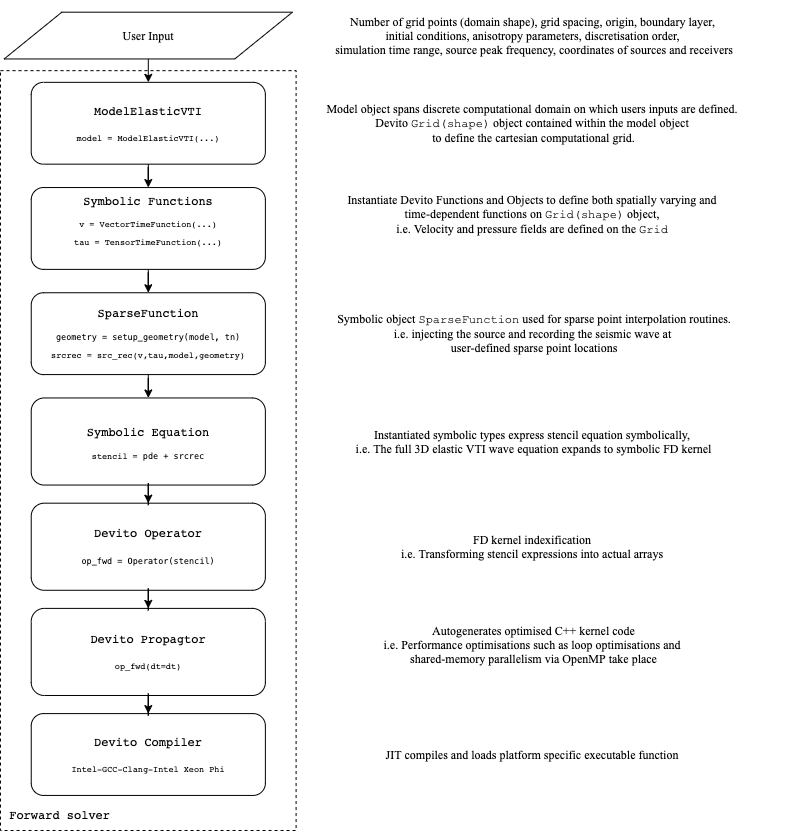
\includegraphics[width=1.0\textwidth]{project/Solver.png}
    \caption{An overview of desired solver architecture}
    \label{fig:solver}
\end{figure}

\newpage
\subsection{Deliverables and timelines}
The GANTT chart in Figure 2 outlines all project tasks, milestones and deliverables.
\begin{figure}[h!]
    \centering
    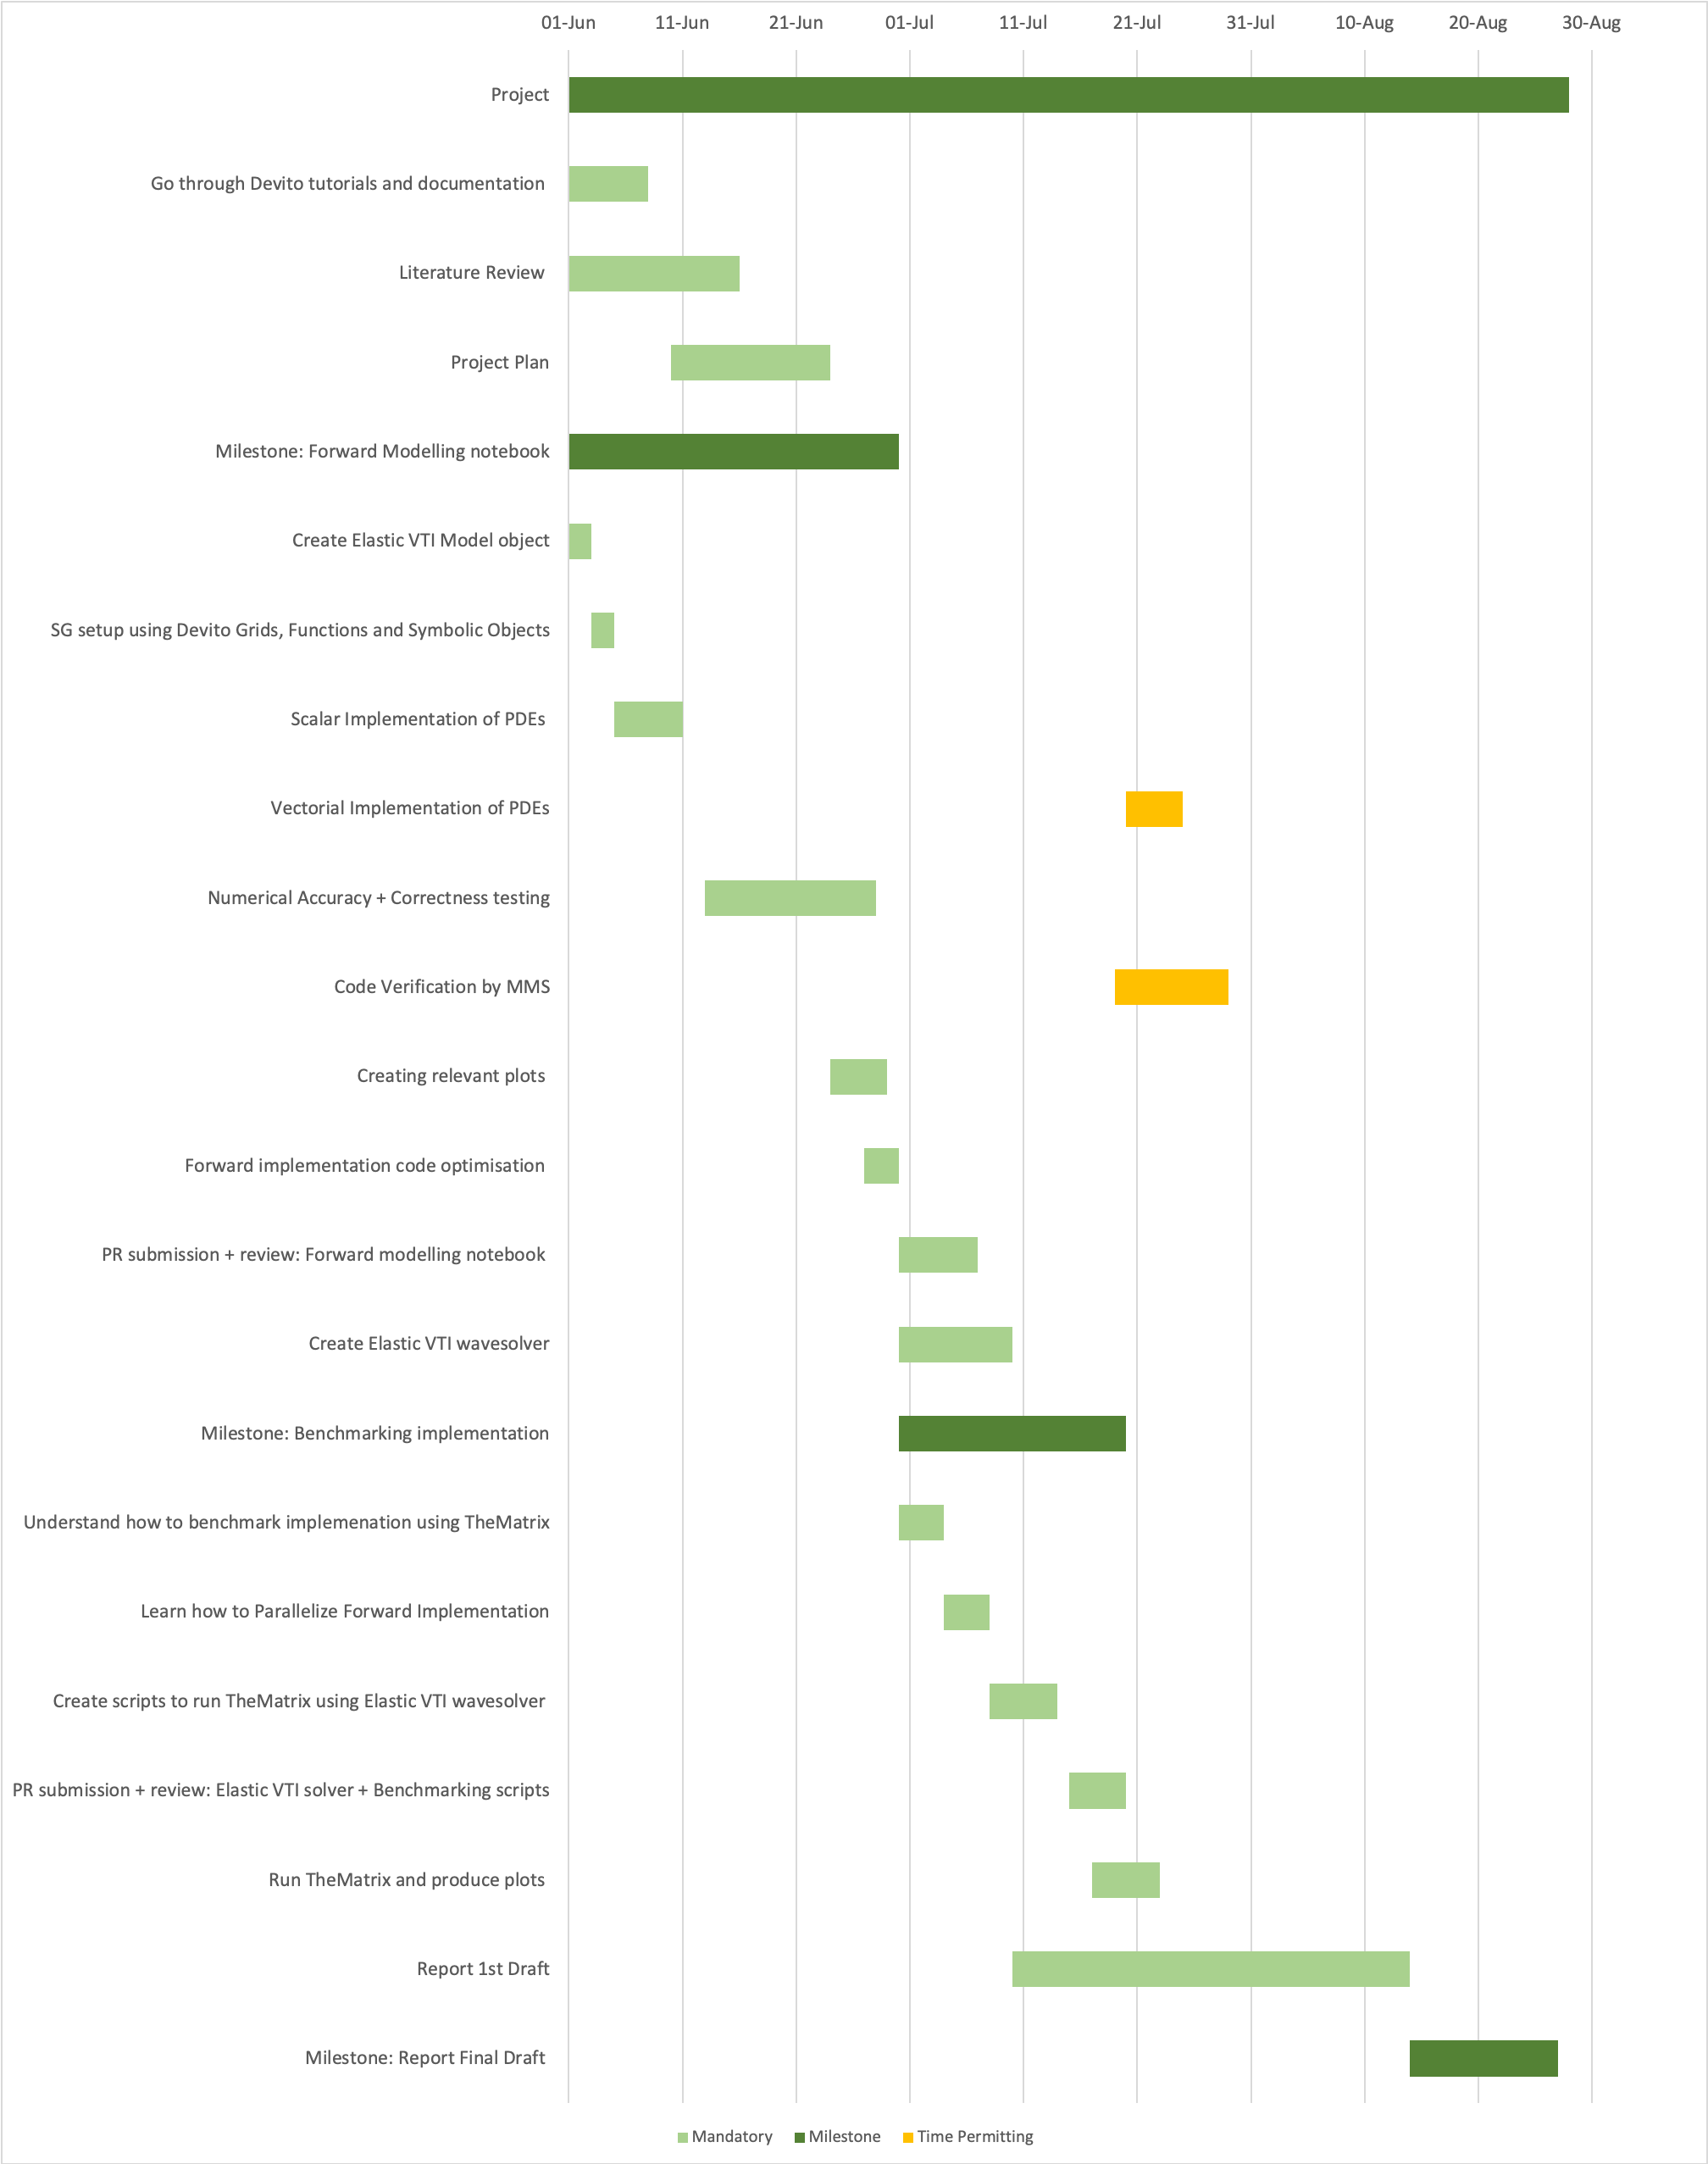
\includegraphics[width=1.0\textwidth]{project/Project_GANTT_Chart.png}
    \caption{GANTT chart illustrating ideal project timeline}
    \label{fig:imperial-picture}
\end{figure}

\newpage
\subsection{Progress to date}
Progress on the project is ahead of the outlined schedule in Figure 2. A notebook outlining how to use Devito to create forward wave propagators using SG-FD scheme to solve the scalar form of the 3D elastic VTI wave equation has been created. At a glance, the implementation seems successful since identical solutions, to the vectorial implementation of the isotropic elastic wave equation are produced when anisotropy is removed from the model, i.e. elastic VTI stress tensor is made purely isotropic. To formally test the robustness and accuracy of the implementation, numerical convergence tests in both time and space are being added to the notebook to ensure the discretisation is stable. An analytical solution has been tested by matching travel times. Parallelly, functions for visualising the model object, plotting receiver shot records, efficiently saving and plotting snapshots to visualise forward wavefield simulation are in development. Furthermore, sample scripts to run the solver on TheMatrix have been added to the graded repository.
\\
\subsection{Acknowledgements}
The Devito Project research group has been exceedingly helpful to solve the day-to-day issues associated with the project, in particular Dr Rohdri Nelson, Dr Mathias Louboutin, Dr Fabio Luporini, Dr Gerard Gorman and Mr. George Bisbas. Without out them, the working forward implementation would not be possible.

